\documentclass[]{article}
\usepackage[paperheight=18cm,paperwidth=18cm]{geometry}
\usepackage{tikz}
\usepackage{pgfplots}
\usepackage{mathrsfs, amssymb, amsfonts}
\pgfplotsset{compat=1.11, width=14cm}
\usetikzlibrary{calc}
\pagecolor{gray}

\tikzset{axis line style/.style={thin, gray, -stealth}}

%opening
\title{Representation of the functions Cos and Sin}

\begin{document}
	
	\thispagestyle{empty}

		\begin{center}
			\huge \color{white} \textbf{The Dance of Cos and Sin}	
			
		\end{center}
	
			\begin{center}
		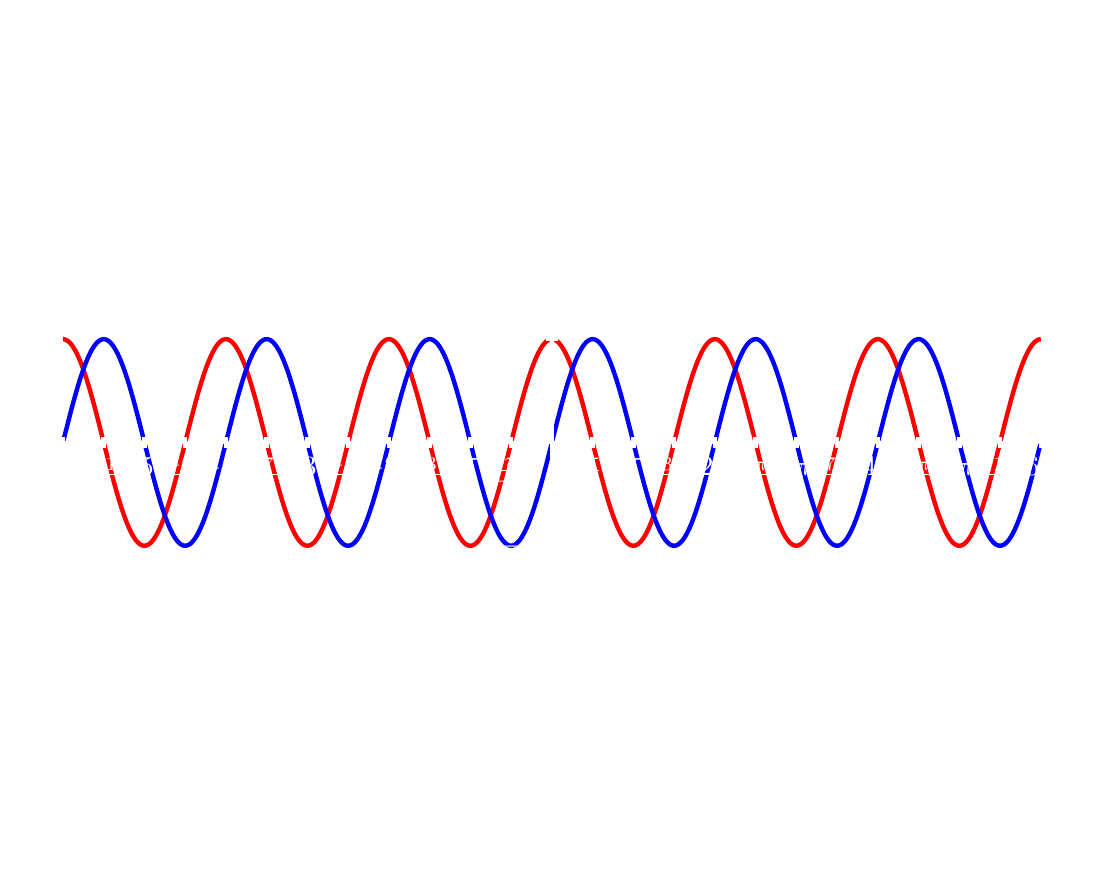
\begin{tikzpicture}
			\begin{axis}[
				axis line style={->, white, very thick},
				xtick={-pi/2,-pi,-3*pi/2,-2*pi,-5*pi/2,-3*pi,-7*pi/2,-4*pi,-9*pi/2,-5*pi,-11*pi/2,-6*pi,0,pi/2,pi,3*pi/2,2*pi,5*pi/2,3*pi,7*pi/2,4*pi,9*pi/2,5*pi,11*pi/2,6*pi}, % Specify the x-tick positions
				xticklabels={$\frac{\pi}{-2}$,$\pi$,$\frac{-3\pi}{2}$,$-2\pi$,$\frac{-5\pi}{2}$,$-3\pi$,$\frac{-7\pi}{2}$,$-4\pi$,$\frac{-9\pi}{2}$,$-5\pi$,$\frac{-11\pi}{2}$,$-6\pi$,0,$\frac{\pi}{2}$,$\pi$,$\frac{3\pi}{2}$,$2\pi$,$\frac{5\pi}{2}$,$3\pi$,$\frac{7\pi}{2}$,$4\pi$,$\frac{9\pi}{2}$,$5\pi$,$\frac{11\pi}{2}$,$6\pi$},xticklabel style={text=white}, tick style={white, ultra thick},
				xlabel= \color{white}$x$,
				ylabel= \color{white}{$y$},
				domain=-6*pi:6*pi,
				samples=1000,
				axis lines=middle, ymin=-4, ymax=4, ytick={-1,1},, yticklabel={$\color{white}\pgfmathprintnumber{\tick}$},
				set layers % Add this line
				]
				
				\addplot[red, ultra thick, on layer=axis background]{cos(deg(x))}; % Specify the layer for this plot
				\addplot[blue, ultra thick, on layer=axis background] {sin(deg(x))}; % Specify the layer for this plot
				
				
			\end{axis}[]
			
		\end{tikzpicture}
		\end{center}
	
	\begin{center}
			\color{white} \small
		\#AEK
	\end{center}
	

\end{document}
